%%%%%%%%%%%%%%%%%%%%%%%%%%%%%%%%%%%%%%%%%%%%%%%%%%%%%%%%%%%%%%%
%
% Phase Diagram for Three Voltmeter Method
%
%%%%%%%%%%%%%%%%%%%%%%%%%%%%%%%%%%%%%%%%%%%%%%%%%%%%%%%%%%%%%%%
% Author: euikook <euikook@gmail.com>  (October 2023)
\documentclass[border=3pt,tikz]{standalone}
%\usepackage{amsmath}
\usepackage{tikz}
\usepackage{physics}
\usepackage[outline]{contour} % glow around text
\usetikzlibrary{angles,quotes} % for pic
\contourlength{1.2pt}

\tikzset{>=latex} % for LaTeX arrow head
\usepackage{xcolor}

\colorlet{veccol}{green!70!black}
\colorlet{vcol}{green!70!black}
\colorlet{xcol}{black!85!black}
\colorlet{projcol}{xcol!60}
\colorlet{unitcol}{xcol!60!black!85}
\colorlet{myblue}{blue!70!black}
\colorlet{myred}{red!90!black}
\colorlet{mypurple}{blue!50!red!80!black!80}
\tikzstyle{vector}=[->,thick,xcol]

\begin{document}
  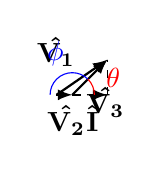
\begin{tikzpicture}[scale=0.1]
    \def\V2{1}
    \def\V3{6.3}
    \def\ang{45}
    \coordinate (V2) at (-2, 0); 
    \coordinate (O) at (0,0);
    \coordinate (V3) at (\ang:\V3);
    \coordinate (I) at ({\V3*cos(\ang)}, 0);

    \draw [vector, ->] (V2) -- (V3) node[midway,left=20,above right=0] {$\vb{\hat{V_1}}$};
    \draw [vector, ->] (V2) -- (O) node[midway,left=10,below right=0] {$\vb{\hat{V_2}}$};
    \draw [vector, ->] (O) -- (V3) node[midway,left=5,below right=0] {$\vb{\hat{V_3}}$};
    \draw [vector, dashed] (O) -- (I) node[midway,left=5,below right=0] {$\vb{\hat{I}}$};
    \draw [dashed] (I) -- (V3);

    \draw pic["$\phi$", blue, draw=blue,angle radius=8,angle eccentricity=2] {angle = V3--O--V2};
    \draw pic["$\theta$", red, draw=red,angle radius=8,angle eccentricity=2] {angle = I--O--V3};

\end{tikzpicture}
\end{document}
